\documentclass[12pt]{article}

%-------------PACKAGES------------- 
\usepackage[margin=1in]{geometry} 
\usepackage{amsmath,amsthm,amssymb}
\usepackage{pgfplots}
\usepackage{float}
\usepackage{braket}
\usepackage{titling}
\usepackage{tikz}
\usepackage{mathtools}
\usepackage{listings}
\usepackage{color}
\usepackage{caption}
\usepackage{subcaption}
\usepackage{algorithm,algpseudocode}
\usetikzlibrary{shapes,arrows,chains}
\usetikzlibrary[calc]

%-------------FORMATTING-------------
\setlength{\droptitle}{-7em} 
\setlength{\parindent}{0pt}
\def\LW{\dimexpr.25\linewidth-.5em} 
\tikzstyle{line} = [draw, -latex']
 
%--------------COMMANDS--------------
\newcommand{\N}{\mathbb{N}}
\newcommand{\Z}{\mathbb{Z}}
\newcommand{\R}{\mathbb{R}}
\newcommand{\C}{\mathbb{C}}
%\renewcommand{\qedsymbol}{\filledbox}

\DeclarePairedDelimiter \abs{\lvert}{\rvert}%
\DeclarePairedDelimiter \babs{\bigg\lvert}{\bigg\rvert}%
\DeclarePairedDelimiter \norm{\lVert}{\rVert}%

%------------ENVIRONMENTS------------- 
\newenvironment{theorem}[2][]{\begin{trivlist}
\item[{\bfseries #1}\hskip \labelsep {\bfseries #2.}]}{\end{trivlist}}
\newenvironment{lemma}[2][Lemma]{\begin{trivlist}
\item[\hskip \labelsep {\bfseries #1}\hskip \labelsep {\bfseries #2.}]}{\end{trivlist}}
\newenvironment{exercise}[2][Exercise]{\begin{trivlist}
\item[\hskip \labelsep {\bfseries #1}\hskip \labelsep {\bfseries #2.}]}{\end{trivlist}}
\newenvironment{reflection}[2][Reflection]{\begin{trivlist}
\item[\hskip \labelsep {\bfseries #1}\hskip \labelsep {\bfseries #2.}]}{\end{trivlist}}
\newenvironment{proposition}[2][Proposition]{\begin{trivlist}
\item[\hskip \labelsep {\bfseries #1}\hskip \labelsep {\bfseries #2.}]}{\end{trivlist}}
\newenvironment{corollary}[2][Corollary]{\begin{trivlist}
\item[\hskip \labelsep {\bfseries #1}\hskip \labelsep {\bfseries #2.}]}{\end{trivlist}}
\newenvironment{definition}[2][]{\begin{trivlist}
\item[{\bfseries #1}\hskip \labelsep {\bfseries #2.}]}{\end{trivlist}}
\theoremstyle{remark}
\newtheorem*{remark}{Remark}

%-------------CODE-STYLE------------
\definecolor{dkgreen}{rgb}{0,0.6,0}
\definecolor{gray}{rgb}{0.5,0.5,0.5}
\definecolor{mauve}{rgb}{0.58,0,0.82}
\lstset{frame=tb,
	language=C++,
	aboveskip=3mm,
	belowskip=3mm,
	showstringspaces=false,
	columns=flexible,
	basicstyle={\small\ttfamily},
	numbers=none,
	numberstyle=\tiny\color{gray},
	keywordstyle=\color{blue},
	commentstyle=\color{dkgreen},
	stringstyle=\color{mauve},
	breaklines=true,
	breakatwhitespace=true,
	tabsize=3
}

\lstset{
	morekeywords={end}
}

%------------------------------------ 
%---------START-OF-DOCUMENT----------
%------------------------------------
\begin{document}
 
\title{Program 5}
\author{David Miller \\ 
MAD5403: Foundations of Computational Math I} 
 
\maketitle

\section{Executive Summary}

Numerical methods for solving ordinary differential equations is of importance in the scientific community, especially computational bioloy. It is important we understand everything about them. In this program we focus on numerical methods for ordinary differential equations. We analyze their error, stability, and convergence as well as implement them. 

\section{Statement of Problem} 

The program consists of three main parts. The first part focuses on a family of linear one step methods and their analysis. We identify well known methods in this family, determine parameters for convergence and $\delta$-dampening, order of convergence, determine regions of absolute stability, and parameters for stiff decay. The analysis is approached from the perspective of characteristic polynomials. \\

The second part of the program focuses on determining and plotting the A-Stability regions for Adams-Bashforth, Adams-Moutlon, BDf, and Linear one step methods. This is also done via characteristic polynomials and the ratio $\rho(\xi)/\sigma(\xi)$. \\

The last part of the program focus on 6 methods
\begin{align*}
	& \textbf{Method 1 - Petzold} : y_n = -4y_{n-1} + 5y_{n-2} + h(4f_{n-1} + 2f_{n-2}) \\
	& \textbf{Method 2 - Explicit Method} : y_n = y_{n-2} + 2hf_{n-1} \\
	& \textbf{Method 3 - Adams Bashforth two-step} : y_n = y_{n-1} + \frac{h}{2}(3f_{n-1} - f_{n-2}) \\
	& \textbf{Method 4 - Adams Moulton one-step} : y_n = y_{n-1} + \frac{h}{2}(f_n + f_{n-1}) \\ 
	& \textbf{Method 5 - BDF one-step} : y_n = y_{n-1} + hf_{n-1} \\
	& \textbf{Method 6 - BDF two-step} : y_n = \frac{4}{3}y_{n-1} - \frac{1}{3}y_{n-2} + \frac{2}{3}hf_n
\end{align*}
where we implement the numerics, perform error and convergence analysis, and determine their stabilities for different parameter values. 

\newpage 

\section{Description of Mathematics}

We use the following theorems and definitions from the class notes

\begin{definition}{Definition 22.2}
	The linear multistep method with cahracteristic polynomials $\rho(\xi)$ and $\sigma(\xi)$ is
	\begin{itemize}
		\item consistent if and only if 
		\begin{align*}
		\rho(1) = 0, \quad \rho^\prime(1) = \sigma(1)
		\end{align*}
		\item satisfies the root conditions if all roots, $\xi_i$, of $\rho(\xi)$ satisfy $\abs{\xi_i} \leq 1$ and roots with unit magnitude are simple 
	\end{itemize}
\end{definition}

\begin{theorem}{Theorem 22.2}
	If a linear multistep method is consistent and satisfies the root condition, then the method is convergent. 
\end{theorem}

\begin{definition}{Definition 22.3}
	A linear multistep method is strongly stable if all of the the roots, $\xi_i$, of $\rho(\xi)$ satisfy $\abs{\xi_i}$ < 1 except the principal root $\xi = 1$.
\end{definition}

\begin{theorem}{Theorem 22.3}
	A strongly stable $k$-step method can have at most order $k+1$.
\end{theorem}

\subsection{Problem 5.1}

A family of linear one step methods is defined by
\begin{align}
	y_n = y_{n-1} + h(\theta f_n + (1 - \theta)f_{n-1})
\end{align}
where $0 \leq \theta \leq 1$. Three well known methods for this family are 
\begin{align}
	& \textbf{Forward Euler} && y_n = y_{n-1} + hf_{n-1} \\
	& \textbf{Backward Euler} && y_n = y_{n-1} + hf_n \\
	& \textbf{Trapezoidal} && y_n = y_{n-1} + 0.5h(f_{n} + f_{n-1})
\end{align}
where Forward Euler has $\theta = 0$, Backward Euler has $\theta = 1$, and Trapezoidal has $\theta = 0.5$. Linear multistep methods are recurrences and can be defined in terms of their characteristic polynomials
\begin{align*}
	\sum\limits_{j=0}^k \alpha_jy_{n-j} & = h\sum\limits_{j=0}^k \beta_jf_{n-j} \\
	\rho(\xi) = \sum\limits_{j=0}^k \alpha_j\eta^{k-j}, \quad \sigma(\xi) = \sum\limits_{j=0}^k &\beta_j\eta^{k-j}, \quad \rho^\prime(\xi) = \sum\limits_{j=0}^{k-1} (k-j)\alpha_j\eta^{k-j-1}
\end{align*}
Using equation (1) we get $\alpha_0 = 1, \, \alpha_1 = -1, \, \beta_0 = \theta,$ and $\beta_1 = 1 - \theta$. From this we arrive at the following characteristic polynomials
\begin{align*}
	\rho(\xi) = \xi - 1, \quad \sigma(\xi) = \theta\xi + 1 - \theta, \quad \rho^\prime(\xi) = 1
\end{align*}
Plugging in the respective values for $\theta$ we ge
\begin{align*}
	\rho(1) = 1 - 1 = 0, \quad \rho^\prime(1) = 1 = \theta + 1 - \theta = \sigma(1) 
\end{align*} 
where these values are actually independent of $\theta$. Thus by Definition 22.2 Forward Euler, Backward Euler, and Trapezoidal are consistent. Also since the only roots of $\rho(\xi)$ si the fundamental unit root, it trivially satisfies the root condition. Therefore Forward Euler, Backward Euler, and Trapezoidal are convergent by Theorem 22.2. It also follows from Definition 22.3 and Theorem 22.3 that these methods are strongly stable and therefore can have at most order 2 on the inerval $0 \leq \theta \leq 1$. \\ 

Considering the test problem $y^\prime = \lambda y, y(0) = C$, a method is called $\delta$-dampening if
\begin{align}
	\lim\limits_{\mathcal{R}(h\lambda)\rightarrow -\infty}\frac{\abs{y_n}}{\abs{y_{n-1}}} \leq \delta
\end{align}
with $0 \leq \delta < 1$. Letting $y^\prime = f \rightarrow h\lambda$ for equation (1) we get
\begin{align*}
	& (1 - h\lambda\theta)y_n = (1 + h\lambda(1-\theta))y_{n-1} \\
	\Rightarrow \quad & \frac{y_n}{y_{n-1}} = \frac{1 + h\lambda(1-\theta)}{1 - h\lambda\theta}
\end{align*}
From which we can derive a relationship for $\delta$-dampening
\begin{align*}
	\lim\limits_{\mathcal{R}(h\lambda)\rightarrow -\infty} \frac{\abs{y_n}}{\abs{y_{n-1}}} = \lim\limits_{\mathcal{R}(h\lambda)\rightarrow -\infty} \babs{1 + \frac{h\lambda}{1 - h\lambda\theta}} = \lim\limits_{\mathcal{R}(h\lambda)\rightarrow -\infty}\babs{1 + \frac{1}{\frac{1}{h\lambda} - \theta}} = \babs{1 - \frac{1}{\theta}}
\end{align*}
Therefore we have for $0 \leq \theta \leq 1$ th following relationship
\begin{align}
	\frac{1}{\theta} - 1 \leq \delta
\end{align}
From equation (6) we can see for $0 \leq \theta < \frac{1}{2}$ that $\abs{y_n} > \abs{y_{n-1}}$ as $\mathcal{R}(h\lambda) \rightarrow -\infty$. This means the solution is an unbounded sequence and thus for this class with $0 \leq \theta < \frac{1}{2}$ can not be A-Stable. Another thing we care about is stiff decay, that is
\begin{align}
	\lim\limits_{\mathcal{R}(h\lambda) \rightarrow -\infty} \frac{y_n}{y_{n-1}} = 0
\end{align}
Taking the absolute value of the limit yields
\begin{align*}
	\lim\limits_{\mathcal{R}(h\lambda) \rightarrow -\infty} \babs{\frac{y_n}{y_{n-1}}} = \frac{1}{\theta} - 1
\end{align*}
Therefore we must have $\theta = 1$ for stiff decay, which is the $\theta$ value for Backward Euler.

\newpage

\subsection{Problem 5.2}

For the A-Stability regions we use the following tables

\begin{figure}[H]
	\centering
	\textbf{Adams Bashforth} \\
	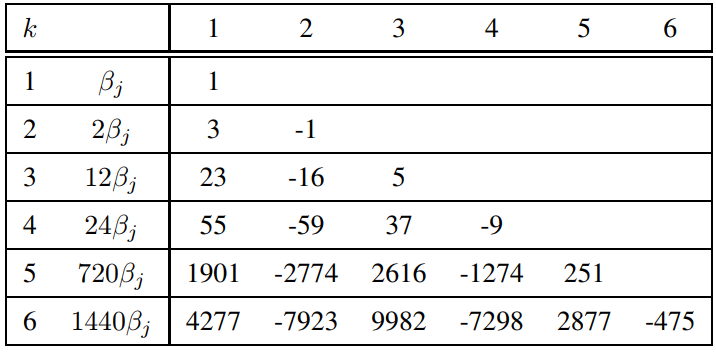
\includegraphics[width=.5\textwidth]{ABTable.png}\hfill
\end{figure}

\begin{figure}[H]
	\centering
	\textbf{Adams Moulton} \\
	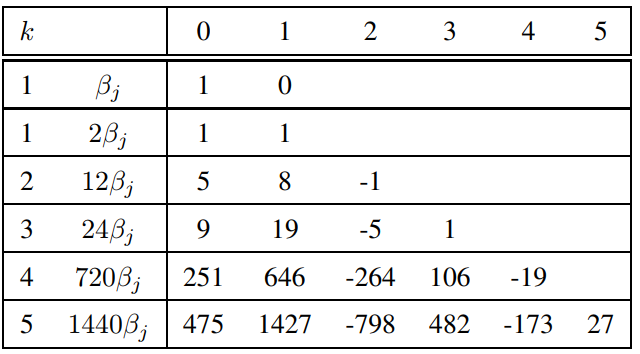
\includegraphics[width=.5\textwidth]{AMTable.png}
\end{figure}
	
\begin{figure}[H]
	\centering
	\textbf{BDF} \\
	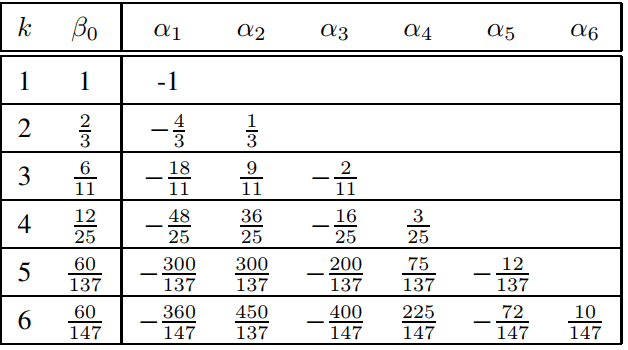
\includegraphics[width=.5\textwidth]{BDFTable.png}
\end{figure}

where we plot the stability regions using the relation 
\begin{align}
	z = \frac{\rho(e^{i\phi})}{\sigma(e^{i\phi})}
\end{align}

\newpage

\subsection{Problem 5.3}

The methods given in this section can are given by the following recurrences
\begin{align}
	& \textbf{Petzold Method (Explicit)} \hspace{7.5cm} \notag \\
	& y_n = -4y_{n-1} + 5y_{n-2} + h(4f_{n-1} + 2f_{n-2}) \\
	\notag \\
	& \textbf{Explicit Midpoint Method (Explicit)} \notag \\
	& y_n = y_{n-2} + 2hf_{n-1} \\
	\notag \\
	& \textbf{Adams Bashforth Two Step (Explicit)} \notag \\
	& y_n = y_{n-1} + \frac{h}{2}(3f_{n-1} - f_{n-2}) \\
	\notag \\
	& \textbf{Adams Bashforth One Step (Implicit)} \notag \\
	& y_n = y_{n-1} + \frac{h}{2}(f_n + f_{n-1}) \\ 
	\notag \\
	& \textbf{BDF One Step (Implicit)} \notag \\
	& y_n = y_{n-1} + hf_n \\
	\notag \\
	& \textbf{BDF Two Step (Implicit)} \notag \\
	& y_n = \frac{4}{3}y_{n-1} - \frac{1}{3}y_{n-2} + \frac{2}{3}hf_n
\end{align} 
where we are given the problem 
\begin{align}
	f = \lambda(y - F(t)) + F^\prime(t), \quad y(0) = y_0 \\
	y(t) = (y_0 - F(0))e^{\lambda t} + F(t)
\end{align}
where $F(t) = \sin(t)$ and $y(0) = 1$ on the unit time domain. Therefore for the implicit methods we can group $y_n$ terms on the LHS with $f_n = \lambda(y_n - sin(t)) + cos(t)$. Therefore the last three methods become

\vspace{0.5cm}

\textbf{IMPORTANT NOTE} : \vspace{.1cm}

It is important to note that Method 1 is the most accurate two-step explicit methods in terms of truncation error, However it does not satisfy the root condition so it is a (terrible) unstable consistent method. Therefore in the results and figures it is omitted since it does not yield anything remotely close to the analytical solution.

\newpage
 
\begin{align*}
	 & \textbf{Adams Moulton One Step Mehtod} \\
	 & y_n = \frac{1}{1 + \frac{h\lambda}{2}}y_{n-1} +  \frac{1}{1 - \frac{h\lambda}{2}}\bigg[0.5h(F^\prime(t_{n-1}) - \lambda F(t_{n-1})) - 0.5h\lambda F(t_n) + 0.5hF^\prime(t_n)\bigg] \\ \\
	 & \textbf{BDF One Step Method} \\
	 & y_n = \frac{1}{1 - h\lambda}\bigg[y_{n-1} - h\lambda F(t_n) + hF^\prime(t_n)\bigg] \\ \\
	 & \textbf{BDF Two Step Method} \\
	 & y_n = \frac{1}{3 - 2h\lambda} \bigg[4y_{n-1} - y_{n-2} - 2h\lambda F(t_n) + 2hF^\prime(t_nj)\bigg]
\end{align*}

\section{Analysis and Design of Algorithms}

For each of the algorithms we have 
\begin{enumerate}
	\item Step size $H$
	\item Left bound $L$ and right bound $R$
	\item Number of points $N = (R - L) / H$
	\item Vector $Y$ which stores numerical results
	\item Initial condition $y(0)$
	\item Function \texttt{f($t_i$, $Y_i$)} from $y^\prime = \lambda f$ and \texttt{exact($t_i$)} for exact solution of the equation
\end{enumerate}

All of the algorithms have $\mathcal{O}(N)$ time complexity and $\mathcal{O}(N)$ space complexity. This comes from the for loop used to compute the vector $Y$ and from having to store the vector $Y$. 

\begin{algorithm}[H]
	\caption{Method 1}
	\begin{algorithmic}[1]
		\State{$Y_0 \leftarrow y(0)$}
		\State{$Y_1 \leftarrow \textbf{exact}(L + H)$}
		\For{$i = 2:1:N$}
		\State{$Y_i \leftarrow Y_{i-1} + 5Y_{i-2} + H(4\textbf{f}(L + (i-1)H, Y_{i-1}) + 4\textbf{f}(L + (i-2)H, Y_{i-2}))$}
		\EndFor \\
		\Return{$Y$}
	\end{algorithmic}
\end{algorithm}

\begin{algorithm}[H]
	\caption{Method 2}
	\begin{algorithmic}[1]
		\State{$Y_0 \leftarrow y(0)$}
		\State{$Y_1 \leftarrow \textbf{exact}(L + H)$}
		\For{$i = 2:1:N$}
		\State{$Y_i \leftarrow Y_{i-2} + 2H\textbf{f}(L + (i-1)H, Y_{i-1})$}
		\EndFor \\
		\Return{$Y$}
	\end{algorithmic}
\end{algorithm}

\begin{algorithm}[H]
	\caption{Method 3}
	\begin{algorithmic}[1]
		\State{$Y_0 \leftarrow y(0)$}
		\State{$Y_1 \leftarrow \textbf{exact}(L + H)$}
		\For{$i = 2:1:N$}
		\State{$Y_i \leftarrow Y_{i-1} + \frac{H}{2}(3\textbf{f}(L+(i-1)H, Y_{i-1}) - \textbf{f}(L+(i-2)H, Y_{i-2}))$}
		\EndFor \\
		\Return{$Y$}
	\end{algorithmic}
\end{algorithm}

\begin{algorithm}[H]
	\caption{Method 4}
	\begin{algorithmic}[1]
		\State{$Y_0 \leftarrow y(0)$}
		\For{$i = 1:1:N$}
		\State{$Y_i \leftarrow \frac{1}{1-H/2}(Y_{i-1} - \frac{H}{2}(\lambda sin(L +iH) - cos(L + iH) - \textbf{f}(L+(i-1)H, Y_{i-1})))$}
		\EndFor \\
		\Return{$Y$}
	\end{algorithmic}
\end{algorithm}

\begin{algorithm}[H]
	\caption{Method 5}
	\begin{algorithmic}[1]
		\State{$Y_0 \leftarrow y(0)$}
		\For{$i = 1:1:N$}
		\State{$Y_i \leftarrow \frac{1}{1 - H/\lambda}(Y_{i-1} - H\lambda sin(L + iH) + Hcos()L + iH)$}
		\EndFor \\
		\Return{$Y$}
	\end{algorithmic}
\end{algorithm}

\begin{algorithm}[H]
	\caption{Method 6}
	\begin{algorithmic}[1]
		\State{$Y_0 \leftarrow y(0)$}
		\State{$Y_1 \leftarrow \textbf{exact}(L + H)$}
		\For{$i = 2:1:N$}
		\State{$Y_i \leftarrow \frac{1}{3 - 2H\lambda}(4Y_{i-1} - Y_{i-2} + 2H(cos(L + iH) - sin(L + iH)))$}
		\EndFor \\
		\Return{$Y$}
	\end{algorithmic}
\end{algorithm}

\newpage

\section{Results and Figures}

\begin{figure}[H]
	\centering
	\begin{subfigure}{.55\textwidth}
		\centering
		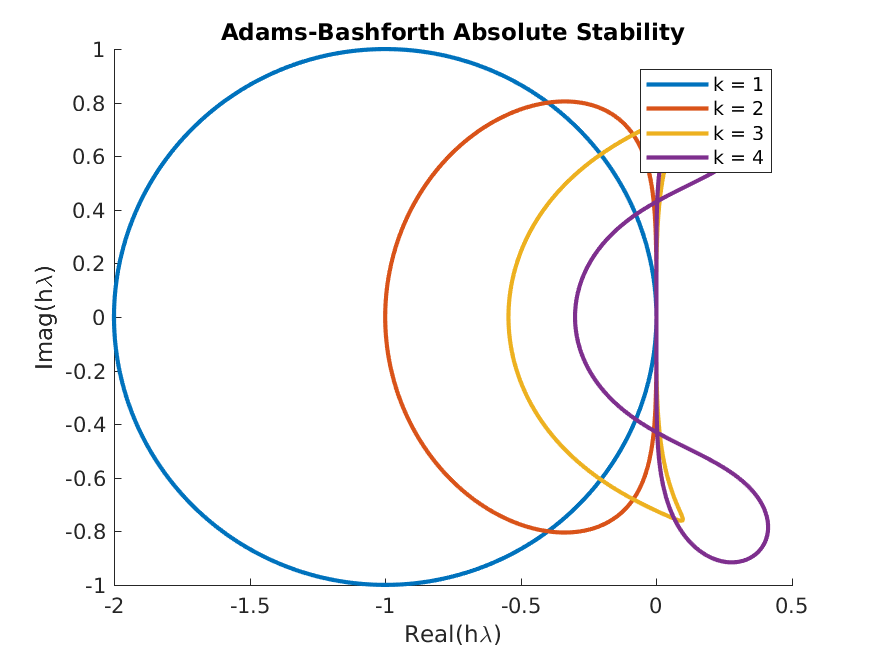
\includegraphics[width=1\linewidth]{5_2_2.png}
		\caption{Adams-Bashforth A-Stability for $k = 1-4.$}
		\label{fig:sub1}
	\end{subfigure}%
	\begin{subfigure}{.55\textwidth}
		\centering
		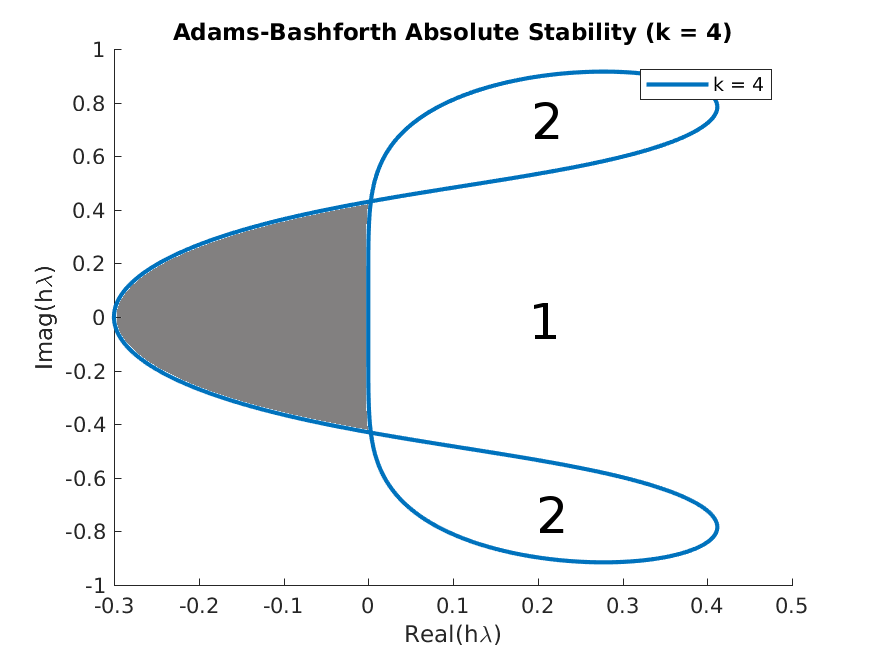
\includegraphics[width=1\linewidth]{5_2_2_single.png}
		\caption{Shaded region is region of A-stability for $k = 4.$}
		\label{fig:sub2}
	\end{subfigure}
	\caption{A-Stability regions for Adams-Bashforth  with stability area shaded in and roots.}
	\label{fig:test}
\end{figure}

\vspace{1cm}

\begin{figure}[H]
	\centering
	\begin{subfigure}{.55\textwidth}
		\centering
		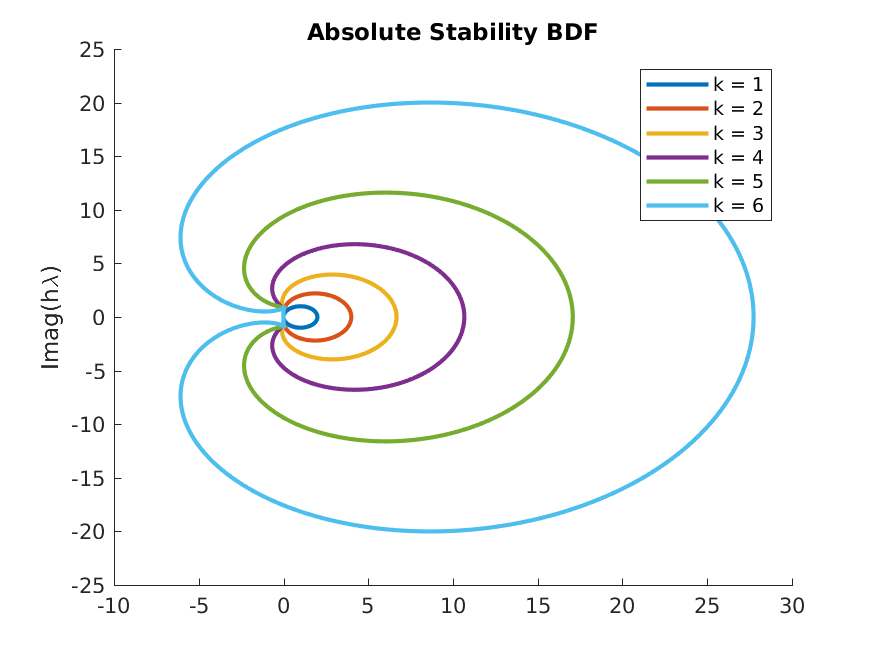
\includegraphics[width=1\linewidth]{5_2_2_1.png}
		\caption{BDF A-Stability for $k = 1-6.$}
		\label{fig:sub1}
	\end{subfigure}%
	\begin{subfigure}{.55\textwidth}
		\centering
		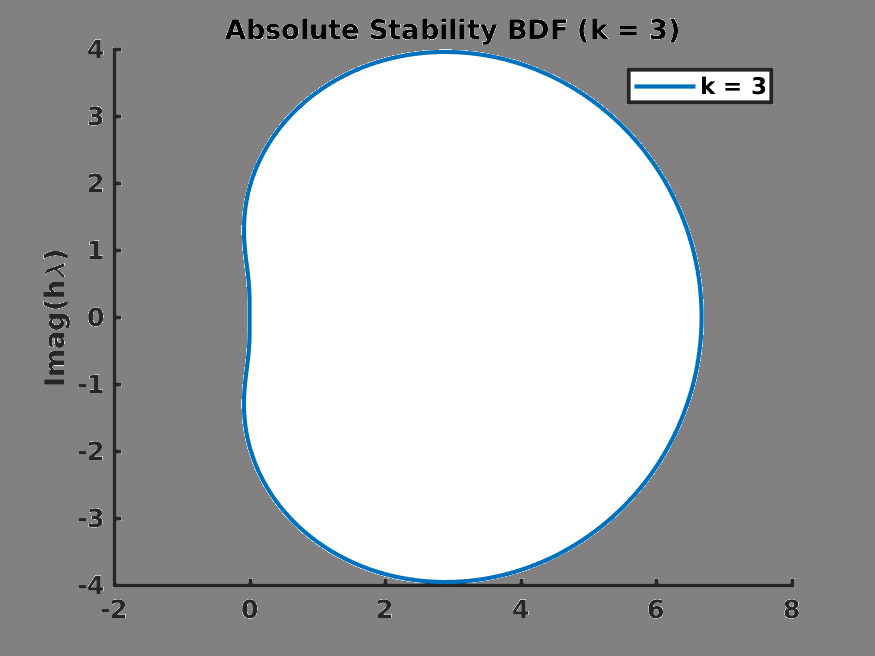
\includegraphics[width=1\linewidth]{5_2_2_1_single.png}
		\caption{Shaded region is region of A-stability for $k = 3.$}
		\label{fig:sub2}
	\end{subfigure}
	\caption{A-Stability regions for BDF  with stability area shaded in and roots.}
	\label{fig:test}
\end{figure}

\begin{figure}[H]
	\centering
	\begin{subfigure}{.55\textwidth}
		\centering
		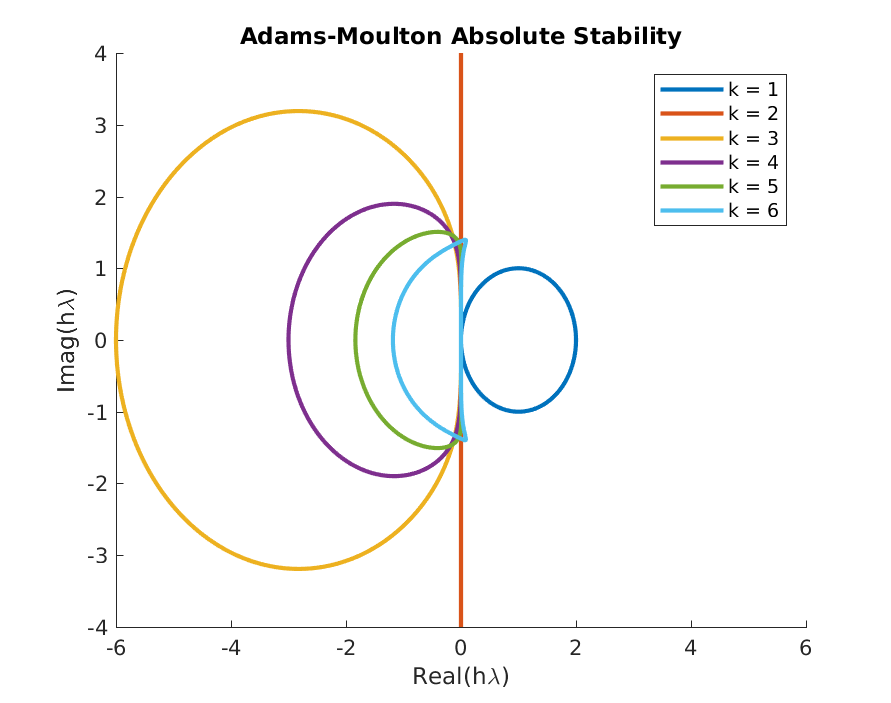
\includegraphics[width=1\linewidth]{5_2_5.png}
		\caption{Adams-Moulton A-Stability for $k = 1-6.$}
		\label{fig:sub1}
	\end{subfigure}%
	\begin{subfigure}{.55\textwidth}
		\centering
		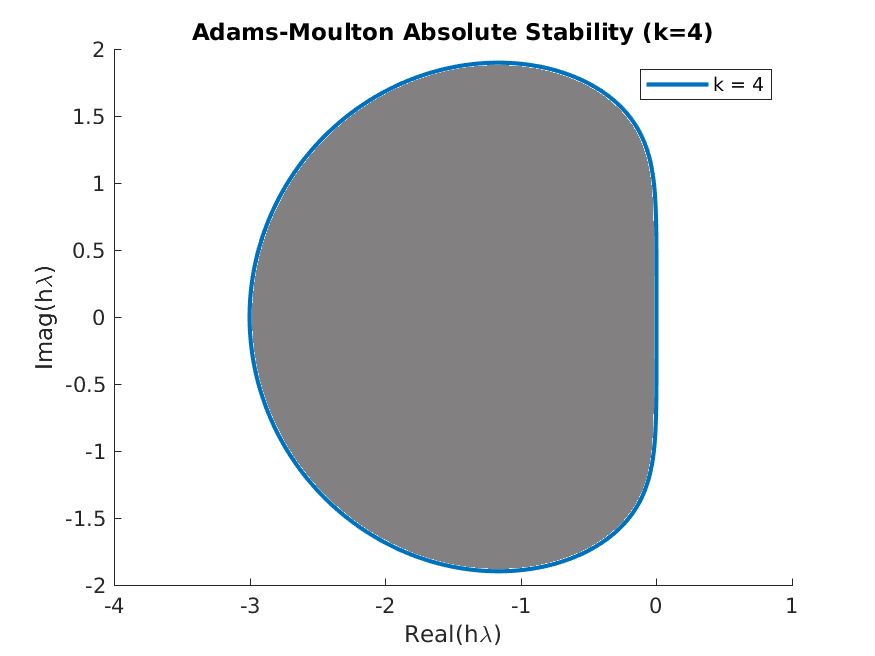
\includegraphics[width=1\linewidth]{5_2_5_single.png}
		\caption{Shaded region is region of A-stability for $k = 3.$}
		\label{fig:sub2}
	\end{subfigure}
	\caption{A-Stability regions for Adams-Moulton  with stability area shaded in and roots.}
	\label{fig:test}
\end{figure}

\begin{figure}[H]
	\centering
	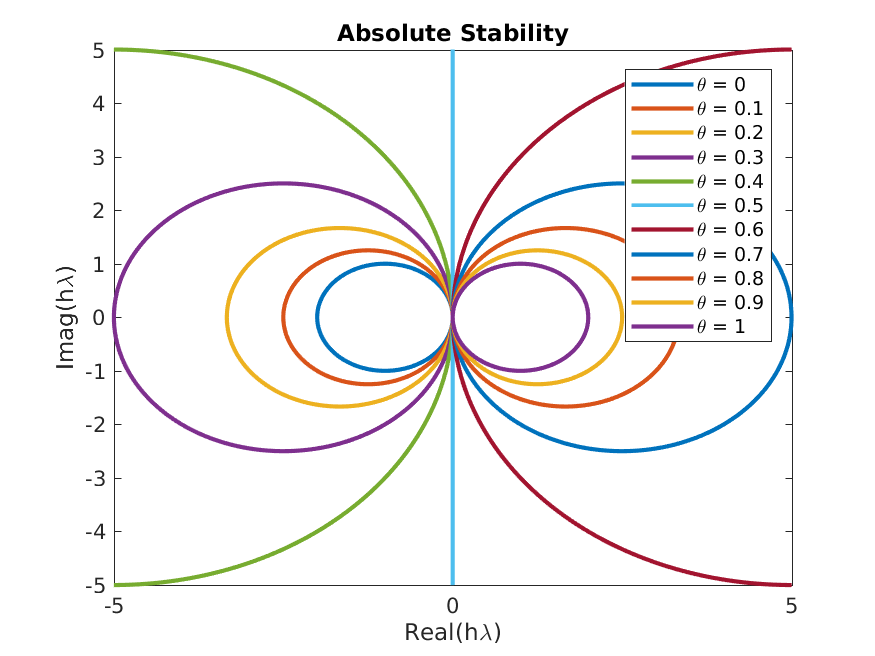
\includegraphics[]{5_2_3.png}
	\caption{A-Stability curves for one step linear methods}
\end{figure}

\begin{figure}[H]
	\centering
	\begin{subfigure}{.55\textwidth}
		\centering
		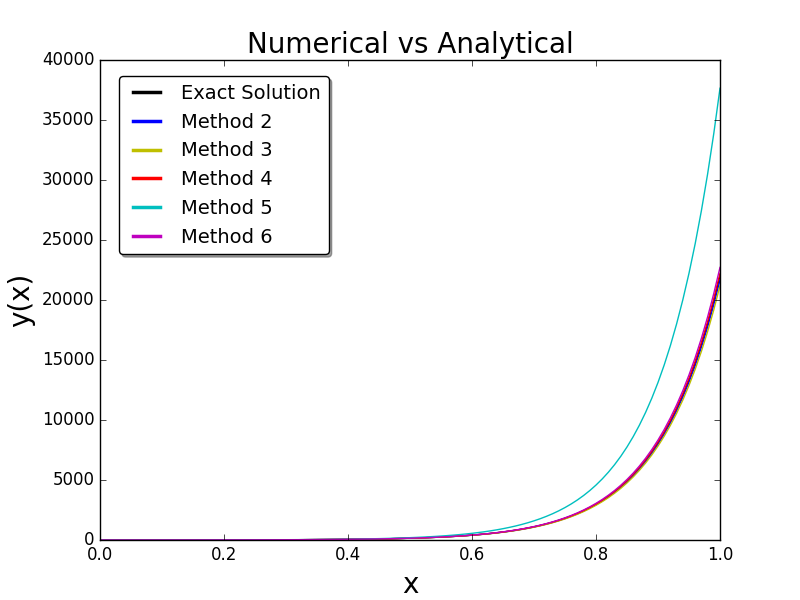
\includegraphics[width=1\linewidth]{reg_10_01.png}
		\caption{Step size $h = 0.01$}
		\label{fig:sub1}
	\end{subfigure}%
	\begin{subfigure}{.55\textwidth}
		\centering
		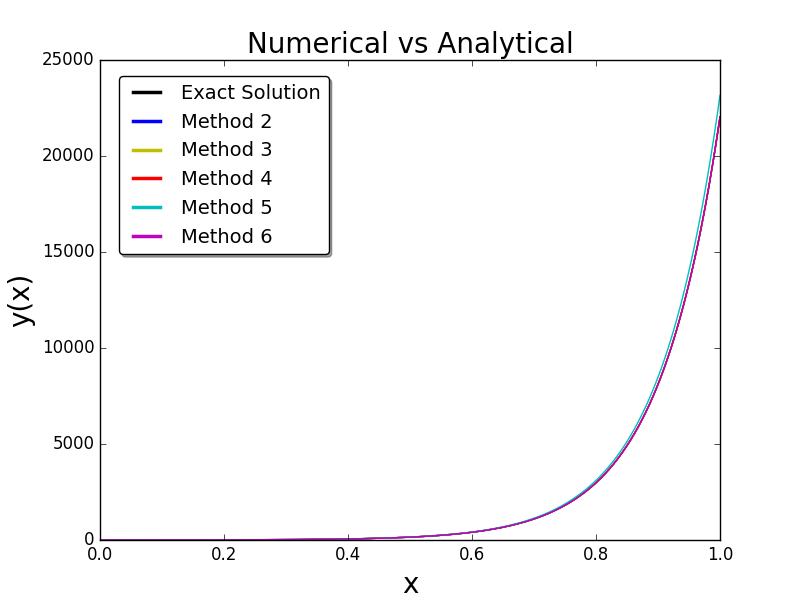
\includegraphics[width=1\linewidth]{reg_10_001.png}
		\caption{Step size $h = 0.001$}
		\label{fig:sub2}
	\end{subfigure}
	\caption{Numerical vs Analytic for $\lambda = 10$}
	\label{fig:test}
\end{figure}

\begin{figure}[H]
	\centering
	\begin{subfigure}{.55\textwidth}
		\centering
		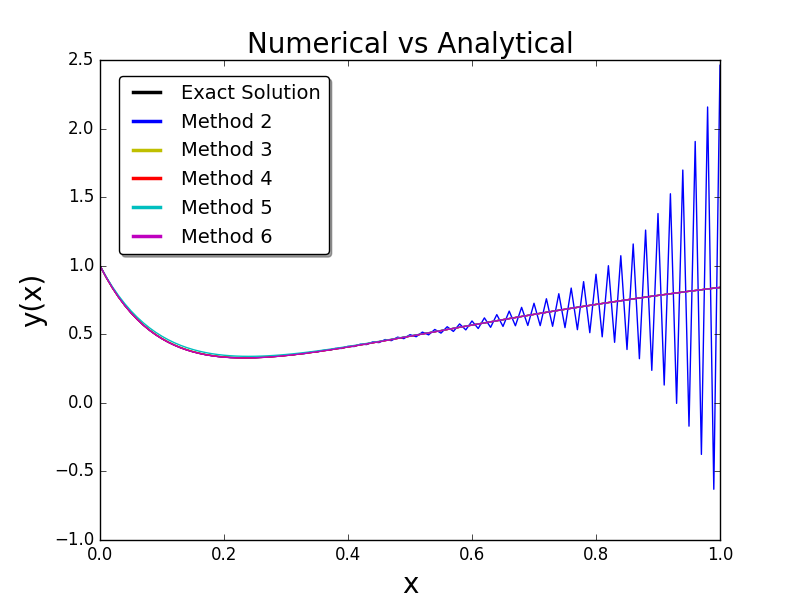
\includegraphics[width=1\linewidth]{reg_-10_01.png}
		\caption{Step size $h = 0.01$}
		\label{fig:sub1}
	\end{subfigure}%
	\begin{subfigure}{.55\textwidth}
		\centering
		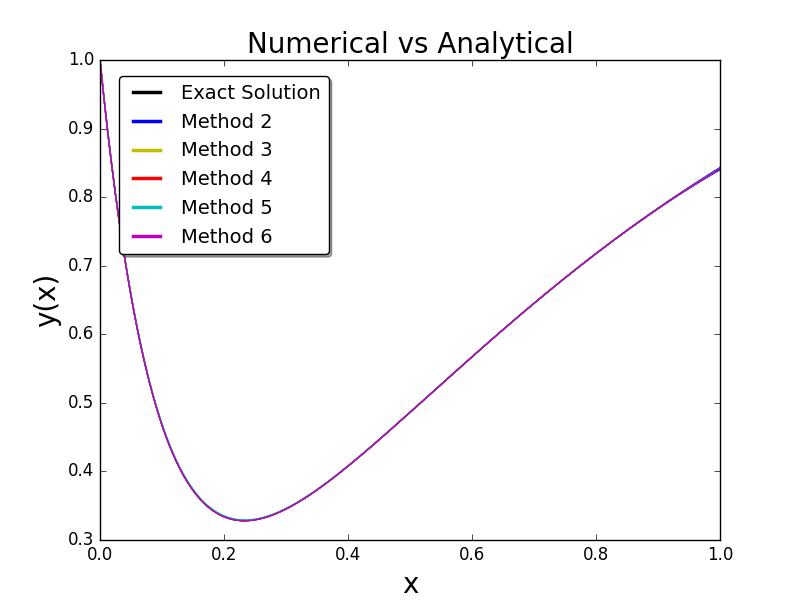
\includegraphics[width=1\linewidth]{reg_-10_001.png}
		\caption{Step size $h = 0.001$}
		\label{fig:sub2}
	\end{subfigure}
	\caption{Numerical vs Analytic for $\lambda = -10$}
	\label{fig:test}
\end{figure}

\begin{figure}[H]
	\centering
	\begin{subfigure}{.55\textwidth}
		\centering
		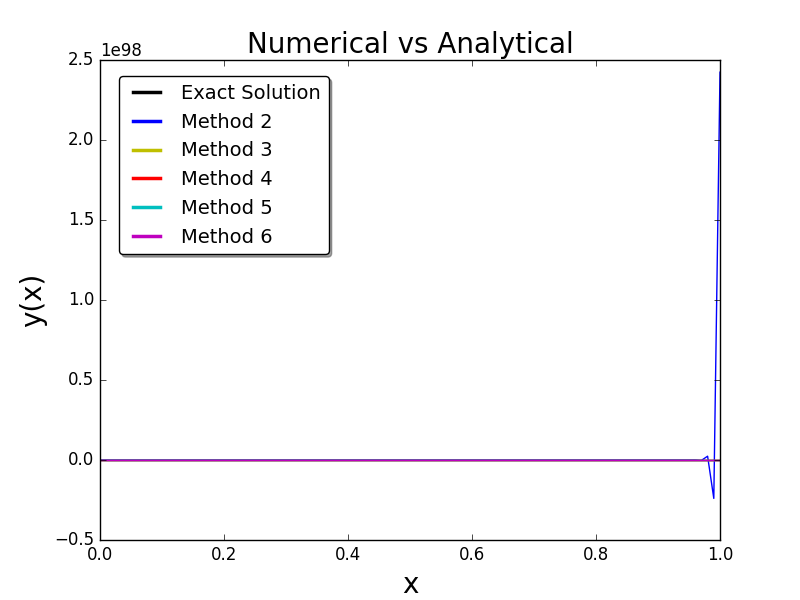
\includegraphics[width=1\linewidth]{reg_-500_01.png}
		\caption{Step size $h = 0.01$}
		\label{fig:sub1}
	\end{subfigure}%
	\begin{subfigure}{.55\textwidth}
		\centering
		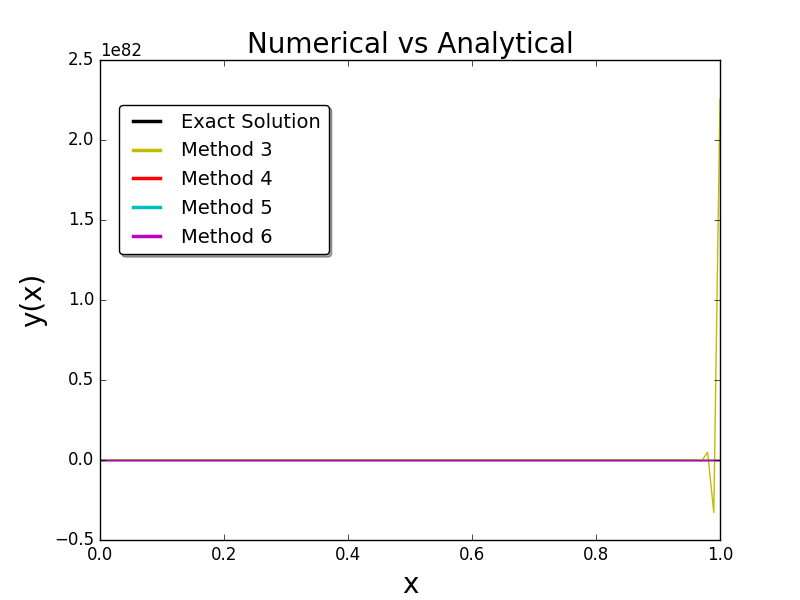
\includegraphics[width=1\linewidth]{reg_-500_01(1).png}
		\caption{Step size $h = 0.01$}
		\label{fig:sub2}
	\end{subfigure}
	\caption{Numerical vs Analytic for $\lambda = -500$}
	\label{fig:test}
\end{figure}

\begin{figure}[H]
	\centering
	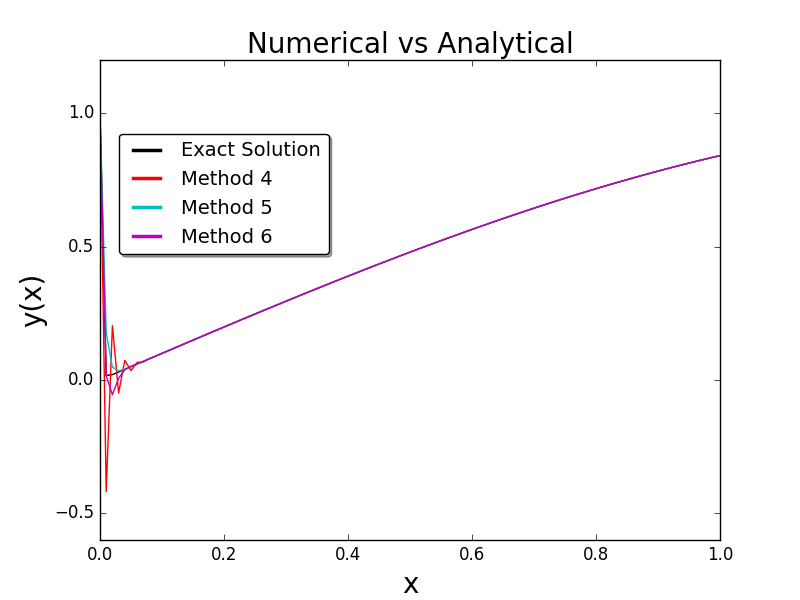
\includegraphics[width=15cm]{reg_-500_01(2).png}
	\caption{Step size $h = 0.01$ and $\lambda = -500$}
\end{figure}

\begin{figure}[H]
	\centering
	\begin{subfigure}{.55\textwidth}
		\centering
		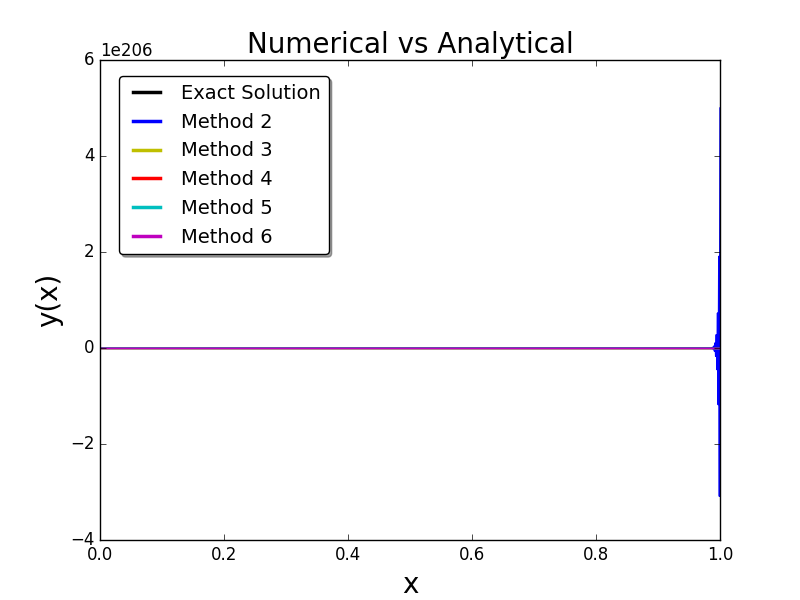
\includegraphics[width=1\linewidth]{reg_-500_001.png}
		\caption{Step size $h = 0.001$}
		\label{fig:sub1}
	\end{subfigure}%
	\begin{subfigure}{.55\textwidth}
		\centering
		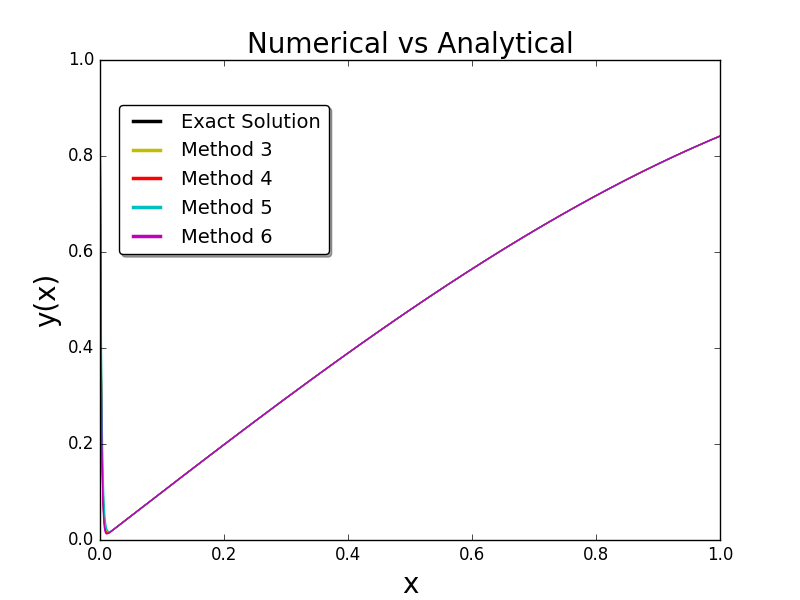
\includegraphics[width=1\linewidth]{reg_-500_001(1).png}
		\caption{Step size $h = 0.001$}
		\label{fig:sub2}
	\end{subfigure}
	\caption{Numerical vs Analytic for $\lambda = -500$}
	\label{fig:test}
\end{figure}

\section{Conclusions}

The numerical results were as we expected from our analysis. Method 1 was terribly unstable and corresponding methods converged once $h\lambda$ was within their stability regions.

\section{References}

I owe credit to the following source for guidance on the code \\

http://math.boisestate.edu/~wright/courses/m566/StabilityDomains/html/StabilityDomains.html

\end{document}
